%% LyX 2.0.0rc3 created this file.  For more info, see http://www.lyx.org/.
%% Do not edit unless you really know what you are doing.
\documentclass[english]{article}
\usepackage[T1]{fontenc}
\usepackage[latin9]{inputenc}
\usepackage{array}
\usepackage{amsmath}
\usepackage{graphicx}

\makeatletter

%%%%%%%%%%%%%%%%%%%%%%%%%%%%%% LyX specific LaTeX commands.
%% Because html converters don't know tabularnewline
\providecommand{\tabularnewline}{\\}

%%%%%%%%%%%%%%%%%%%%%%%%%%%%%% User specified LaTeX commands.
\usepackage{color}
\usepackage{graphicx}

\@ifundefined{showcaptionsetup}{}{%
 \PassOptionsToPackage{caption=false}{subfig}}
\usepackage{subfig}
\makeatother

\usepackage{babel}
\begin{document}

\title{Bending and Torsion Minimization of Toroidal Loops}


\author{Avik Das, Victor Huang\\
Adviser: Carlo S�quin\\
\\
\emph{CS Division, University of California, Berkeley}}
\maketitle
\begin{abstract}
We focus on a special optimization problem of parameterized surfaces of genus one.
In particular we trade off the penalty functions for bending a toroidal path 
and for applying a twist to it and aim to find local minima of this cost function.
This analysis forms a key element in demonstrating the different regular homotopy classes of tori.
A generalization of this surface optimization, which considers curvature
as well as any shearing of its parameter grid, may be used to find
the most optimal direct path from an arbitrary closed manifold of genus one
into one of the four basic representatives of four regular homotopy classes of tori.\\


\emph{key words}: torus, bending energy, twisting energy, gradient descent, regular homotopy.
\end{abstract}

[[USE A MORE PAGE-FILLING FORMAT -- I.E. A LINE WIDTH OF AT LEAST 6 INCHES ]]

\section{Problem Statement and Background}

We study minimum-energy configurations of toroidal surfaces.
In this report we are only concerned with simple sweeps of a constant (circular) cross section
along a smooth, closed sweep path.
As this sweep path changes its shape in 3D space, the integrated torsion around its loop changes ( \ref{fig:torsion} ).
The absolute value of this integrated torsion is determined by generating a sequence
of rotation minimizing frames (RMF) \cite{bishop75} \cite{klok86} \cite{wang97} \cite{wang08} 
along the curve and measuring the misalignment
between an arbitrary starting frame and the end-frame that is being generated by going once around the toroidal loop.
For a planar sweep curve with no inflection points the overall torsion is always zero ( \ref{fig:torsion}a ),
since the RMF will always keep its bi-normal axis perpendicular to the plane of the sweep curve.

[[When regenerating all the figures, please avoid the Mathematica-kind of colored directional illumination.
We want to clearly see four different hues on four different sides of the toroid, so that the twist stands out easily.]]

FIGURE 1
%\caption{\label{fig:torsion}

Figure 1: Loops with and without overall torsion: 
(a) A 3D space curve will typically have some built in torsion [[Fig.1c -- but a more obvious 3D configuration]];
(b) in space curves with the proper kind of symmetry, the overall torsion can cancel out to zero [[Fig. 1b]];
(c) in planar curves without inflection points the overall torsion is always zero [[Fig. 1a]].




If such a loop ( \ref{fig:torsion}a ) is smoothly deformed through a warped 3D configuration
into some figure-8 shape, where the approaching path segments are allowed to cross over each other ( \ref{fig:cro0ssover}b ),
and is then further deformed until it forms again a roughly circular, planar path ( \ref{fig:cro0ssover}c ),
then we find that the overall torsion has changed by exactly +/- $720^{\circ}$.


FIGURE 2
%\caption{\label{fig:crossover}

Figure 2: A figure-8 cross-over move will add or subtract $720^{\circ}$ of torsion: 
(a) Circular starting configuration with zero torsion;
(b) Figure-8 configuration with $360^{\circ}$ of torsion;
(c) circular end configuration with $720^{\circ}$ of torsion.



An immersion of a 2-manifold into $\mathbb{R}^3$ implies that the neighborhood around every point of this surface
is equivalent to a small disk.
Thus the surface must not have any tears, creases, or pinch-off points.
On the other hand, we are allowed to deform the surface smoothly as much as we like
and let it self-intersect and pass through itself as often as we like.
A transformations of this kind that also leaves any parameterization grid on this surface
connected at all times is called a regular homotopy.
It is known that all orientable surfaces of genus one fall into four different classes
that cannot be transformed into one another with a regular homotopy  \cite{hass85}.
An easy-to-understand introduction to these four homotopy classes of tori
and a visualization of four simple representatives for these classes can be found in \cite{sequin11}.

The goal of this project is to find local minima in the combined penalty functions 
for bending and for twisting of simple toroidal shapes 
and to generate some visualizations of the deformation sequences that would lead to these minima.
To keep things simple and to allow the optimization to progress at interactive speeds,
we choose a very structured representation of the tori with relatively few independent parameters.
We simply use an abstract representation of a piece-wise linear sweep path 
enhanced with a sequence of rotation-minimizing frames.
The overall bending energy is calculated as the sum of the squared turning angles
at the joints of subsequent line segments along the sweep path.
The overall twist energy is simply proportional to the squared value of the overall torsion.
By selecting the relative weights for these two energy components,
we can choose to obtain either circular loops with some possible non-zero overall torsion,
or some true 3D space curve with a lesser amount of overall torsion.
A gradient-descent optimization loop will push a given toroid with some built-in twist
into the nearest local minimum.
These issues are discussed in more details in the subsequent sections
and visualization models for several gradient-descent optimization runs are presented.


[[THIS GETS REPLACED BY ABOVE FIGURES ]]

\begin{figure}
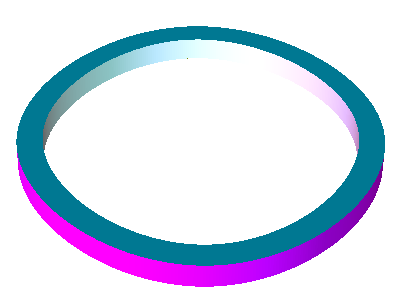
\includegraphics[width=1.5in]{untwisted-circle-1-smooth}\hfill{}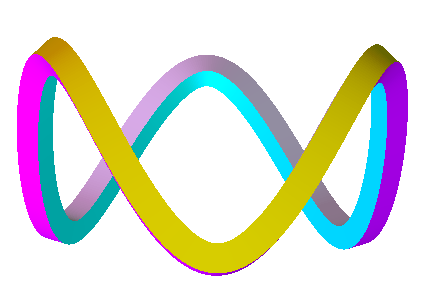
\includegraphics[width=1.5in]{wavy-1}\hfill{}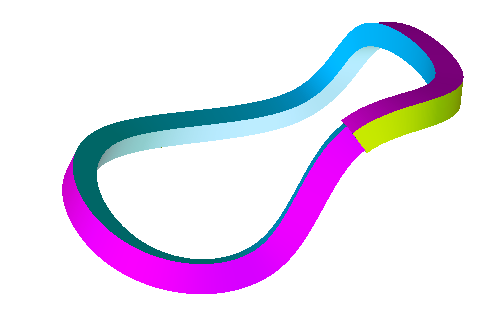
\includegraphics[width=1.5in]{twisty-1}

\caption{Various space curves with and without cross-sectional mismatch}
\end{figure}


\begin{figure}
\hfill{}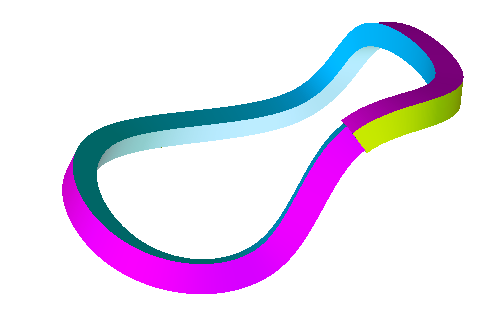
\includegraphics[width=1.5in]{twisty-1}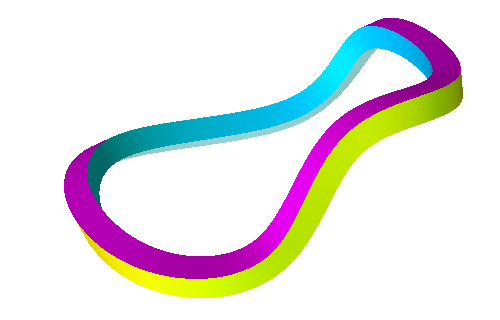
\includegraphics[width=1.5in]{twisty-1-compensated}\hfill{}

\caption{Cross-sectional mismatch compensated by a twist}
\end{figure}



\section{Toroid Representation and Energy Functionals}

The sweep path of the toroid is rendered as a closed B-spline,
regularly sampled in parameter space with a user-definable number of segments.
The few control points of the B-spline allow the user to define the geometry of the starting configuration.
The end-to-end torsion is then calculated, 
and some compensating twist is introduced to generate properly aligned end-frames.
Any artificially introduced twist is uniformly spread out over the whole parameter range of the complete spline curve.
The user can also optionally introduce additional twist.
In most cases this twist will be a multiple of $360^{\circ}$, 
since we want to make sure that our surface corresponds to a torus with proper parameterization, 
in which all parameter lines close onto themselves if one goes once around the loop 
(or around the minor circle as well).
As the sweep curve is deformed gradually, 
the overall twist is adjusted incrementally from one iteration to the next,
to guarantee that the end-to-end connectivity of the torus does not suddenly change 
by taking a jump in twist of +/- $360^{\circ}$.

The energy functional used in the various optimization runs is composed of three parts.
They have been designed to preserve the length of the sweep curve (approximately),
and to measure its total bending energy and twist energy, respectively.


\subsection{Representation}

Even though the sweep curve is rendered as a "smooth" B-spline
(depending on how many line segments the user is asking for),
all calculations of energy and all optimization moves are simply carried out on the control polygon.
This reduces dramatically the degrees of freedom in the system and 
the scale of the derivative computations in the optimization process.
An edge between two subsequent control vertices is called a \emph{strut}, 
with the $i$th strut denoted as the vector $S_{i}$ in the following calculations.


\subsection{Spring Energy}

To keep the curve length roughly the same as originally drawn and to avoid tedious rescaling steps, 
the average length of all the initial struts $\left\Vert S_{i}\right\Vert$
is defined to be their desired rest length $R$ during the optimization process.
Understanding the struts as idealized springs, 
the square of the deviation from the rest length $R$ is proportional to the energy stored in these springs,
and the sum of these terms is used as one component of the cost function during optimization.
Applying Hooke's Law with a spring constant $k$ leads to the following energy term:
\[
E_{S} = \sum_{i}\frac{1}{2}\cdot k\cdot(\left\Vert S_{i}\right\Vert - R)^{2}
\]


\subsection{Bending Energy}

Common approaches to calculating the bending energy of a 2-manifold
typically consider the curvature of the surface at each point integrated over the entire surface.
Since our study concentrates on thin, tube-like structures with a constant cross section,
we restrict ourselves to considering only the amount of bending found in the sweep path itself.
Unfortunately, the bending energy of a smooth curve,
calculated as an arc-length integration of curvature squared,
is not scale invariant.
However, since we work only with a coarse, discrete representation of our curve, 
i.e., the control polygon of a B-spline, 
and since we have a separate mechanism to maintain the lengths of the individual curve segments
(see previous subsection),
we can also calculate the bending energy in discrete form,
based on the turning angles at all the joints of the control polygon.
Each joint contributes the square of its deviation from collinearity:
[[ There is no reason to flip one of the two vectors backwards; use them in their natural forward-pointing direction !]]

\[
E_{B} = \sum_{i}\left(\arccos\left(\frac{S_{i-1}\cdot S_{i}}{\left\Vert S_{i-1}\right\Vert \cdot\left\Vert S_{i}\right\Vert }\right)\right)^{2}
\]

%[[We do not need these extra explanations ...]
%The calculation of the inverse cosine of the normalized dot product
is the standard calculation of the angle between two vectors, with
the assumption that both vectors have their tail at a common point.
In our case, this means that both struts have their tail in the middle
of three neighboring vertices and point toward the other two. This
angle is then substracted from the optimal $180^{\circ}$, which would
be angle between the two struts if all three vertices were colinear.
Finally, the square of this deviation is summed across the curve.

%This formulation of the bending energy suffices because the shape
of the cross-section of the object in question is constant, and thus
only the sweep of the curve itself is used to compare two objects
with respect to their energies. Note that this implies a Clifford
torus need not be achieved if a topologically equivalent shape is
optimized, and in fact the optimal in that case is the unit circle,
regardless of the cross-section used to render the shape.


\subsection{Twist Energy}

Since we are interested not just in the pure geometrical shape of a toroid under investigation,
but also in the deformation of a parameter grid embedded in its surface,
we have to add a third term to our cost function: the twist energy.
This is a measure of the deviation of a given state of the toroid
from the geometry produced by a pure RMF (rotation minimizing frame).

The framework used for the generation and optimization of these toroidal shapes
uses by default an RMF along the control polygon.
Despite the fact that both the starting and ending cross-sections 
are sampled at the same point on the curve, 
the incremental forward projection of the RMF, 
calculated as per Wang et al. \cite{wang97} \cite{wang08},
may result in a mismatch between the two cross-sections. 
The normal vectors to the curve within the two cross-sections are compared to each other, 
and the angle between these two vectors measures the mismatch between the two coordinate frames.
The framework can then apply an additional global twist to the whole curve, 
so that the beginning and ending coordinate frames line up
and the longitudinal parameter lines in the toroid surface 
properly join with themselves after one pass around the loop.
This additional twist is distributed evenly among all line segments of the sweep path; 
thus with a global twist of $t$ and with $n$ sampled cross-sections,
the local twist along each of the $n$ line segments is $\frac{i}{n}\cdot t$. 
After a match of the two end-frames has been established,
the user can add additional global twist in increments of +/- $360^{\circ}$,
which keeps all longitudinal parameter lines properly connected to themselves.

The simplest way to define a twist penalty is to use the square of this total twist,
comprising the component needed to establish the matching coordinate frames
as well as any additional twist added by the user.
\[
E_{T} = \text{Built-in curve torsion} + \text{user-added twist}.
\]
Once this toroidal end-around connectivity has been initialized,
it is important that it be maintained throughout the whole optimization process.
Thus the global twist is updated incrementally after each change to the curve shape,
so that the two end frames keep their alignment.
This prevents the toroid from suddenly experiencing jumps in twist of +/- $360^{\circ}$,
as the framework looks for a minimal amount of global twist to keep the two coordinate frames aligned.

However, this simple calculation of a twist penalty may not be quite good enough.
Even though for many optimization sequences studied,
this functional was good enough to guide the toroid evolution to the expected final state,
there were some cases where this optimization process passed through some highly convoluted shapes.
In a continuation of this project we will thus have to consider a more refined assessment
of the twistiness of the whole toroid, - one that does not allow heavily twisted segments
with opposite signs in their overall torsion to cancel out.
We thus need to find a way to calculate the twist along each segment independently
by monitoring how much the normal vector in the Frenet frame 
(the natural intrinsic coordinate system based on local curvature)
changes from one joint to the next.

[[I have used the occasion of this re-writing pass to think deeply about this issue.
Here is my current thinking. Please bring your thoughts to the table.
And then finally this needs to be verified by an experimentally.]]

However, this is a somewhat tricky issue.
Just considering the rotation angle from one frame to the next may lead to a hyper-sensitive, discontinuous functional.
When a control point in a planar curve moves slightly so as to introduce two inflection points,
the Frenet frame suddenly flips through $180^{\circ}$ at these inflection points, 
which would add a huge penalty to the cost function and
may trigger instabilities in the optimization process.
But we really do not want to introduce any hurdles for almost straight curve segment sequences with a possible inflection point in it.
Thus any frame rotation around the tangent direction must be seen in the context of curve bending;
and this rotational cost component should be weighted by the bending cost.
Thus the local twist cost can pass gracefully through a value of zero 
as two subsequent curve segments pas through a collinear configuration.
Thus a refined form of the twist cost component may amount to:
\[
E_{3} = \sum_{i}\left(\frac{S_{i-1}\cdot S_{i}\times S_{i+1}} 
{\left\Vert S_{i-1}\right\Vert \cdot\left\Vert S_{i}\right\Vert \cdot\left\Vert S_{i-1}\right\Vert } \right)^{2}
\]
Another way of looking at this cost component is to see it as a penalty for non-planarity of 3 subsequent curve segments.
And perhaps this is the best way of expressing local twistiness; 
because creating a helical path is one way of absorbing some built-in twist without incurring a twist penalty for it.
However the energy component $E_{3}$ would discourage such a diversion of a curve into a 3D configuration
(see discussion in subsection "Undesirable Behavior").


\subsection{The Combined Functional}

For the purposes of investigating the effect of penalizing twist,
the amount of penalty incurred by the twist is controllable by the
user. Then, given a spring energy $S$, a bending energy $B$ and
a twist energy $T$, the final energy of the shape is
\[
E = E_{S} +(1-\alpha)\cdot E_{B} + \alpha\cdot E_{T} + (optionally) \beta\cdot E_{3}
\]
First the spring constant $k$ in $E_{S}$ is adjusted so that obtaining struts
that are all close to the rest length has priority over any other adjustments to the control points,
without making the optimization problem too stiff.
[[WHAT WAS A GOOD VALUE THAT ACHIEVED THIS ?]]
Then the user can play with the parameter $\alpha$, which trades off the twist penalty weight against bending costs.
Adjusting this ratio is the primary way to affect the outcome of the optimization.
Experimenting with parameter $\beta$ in the future should reveal how easy it is to suppress the unwanted formation of local helices.


\section{Optimization}


\subsection{Gradient Descent}

A standard gradient descent algorithm is used to optimize the given input toroid
by minimizing the energy of the final configuration. While an analytic approach
to solving a set of linear equations using gradient descent is possible,
this type of analytic approach is not well suited to minimizing our energy
functional. Firstly, the bending energy components by themselves are already
difficult to analyze in closed form. Secondly, the twist energy is
determined by the numerical method of approximating the RMF using
a sequence of frames sampled along the curve, and the accumulation
of twist is calculating by updating a parameter that is used in the
calculation of the change in twist in subsequent iterations 
- a process that is difficult to capture in closed form. 

Thus, we employ finite differencing to determine the influence of each primary parameter 
on the overall cost of the resulting configuration.
Each parameter, in our case: each coordinate component of each control point, is varied
independently by a small amount, and the resulting change in the energy of the toroid is calculated.
Given a sweep curve defined by $n$ control points, there are a total of $3n$ parameters.
Each of these parameters $p_{i}$ is first changed by an amount $+\Delta p$, resulting in a new toroid energy $E^{+}$,
and subsequently by $-\Delta p$, resulting in a toroid energy $E^{-}$.
Thus, the impact of the $i$th component on the toroidal energy is 
\[
\Delta E_{i}=\begin{cases}
E^{-}-E^{+} & E^{-}<E^{0}\text{ or }E^{+}<E^{0}\\
0 & \text{otherwise}
\end{cases}
\]
where $E^{0}$ is the energy of the shape before the parameter is varied. 
With this approach the overal energy gradient can be calculated as:
$\Delta E / 2\cdot\Delta p = <\Delta E_{1},\ldots,\Delta E_{3n}> / 2\cdot\Delta p $;
and this vector will point in the direction of the largest decrease in energy, with
each parametric components weighted by the magnitude of the energy decrease due to that parameter. 

[[The following is not a good thing: the "test step size" for finite differencing
and the step size to be taken in the energy landscape should be kept separate.
Also don't confuse a change in energy with the "gradient" which is delta e / delta p ! ]]

%The gradient is then normalized so its magnitude is the
step size, $\Delta p$, and this change is applied to the parameters
to produce the result of the current iteration.


\subsection{Step Size}

Both, the amount by which parameters should be varied to reliably calculate the energy gradient vector, 
as well as the distance along that vector that should be traveled in one iteration, 
are crucial to an efficient and stable optimization process. 
In addition, if we are interested in creating a real-time interactive visualization or a smoothly evolving demonstration movie,
additional constraints on the step size and thus on the optimization speed, may come into play.

For the purposes of this project, 
the initial finite-differencing step is set at [[WHAT?]].
The initial optimization step size is set at [[WHAT?]].
Before each iteration step is carried out, it is checked that 
the intended step would indeed result in a reduction in the overall energy function.
If this is not the case, the iteration step size is cut in half,
and subsequent iterations attempt to decrease the energy by using this new, reduced step size. 
When the step size drops below a predefined ending step size, [[HOW IS THIS SET?]]
the optimization halts, and it is inferred that the toroid has reached a local optimum.

The iteration step size has an important influence on the progress of the optimization.
Too large a step size may result in flying past one local minimum into a
valley containing another local minimum of possibly higher energy,
or it may cause tunneling through a barrier into an inappropriate region of the energy landscape.
Too small a step size may result in unacceptably long convergence times.

One often-used optimization approach is to employ a line search algorithm, %\cite{??}, 
in which the direction of the gradient is searched in a more refined manner
to find an appropriate energy minimum on that line.
This algorithm was not used for this project. 
A first reason was simplicity and that fact that satisfactory results were obtained
with a straight-forward gradient-descent algorithm.
But another concern was also that such a line-search algorithm may result in a rather uneven rate of progress.
This would be rather undesirable when trying to create real-time interactive visualizations
or smoothly progressing movies of the evolution of a toroidal shape.



\section{Results}

\subsection{Elementary Test Cases}

The most fundamental benchmark for this project is the unfolding of
a planar, untwisted figure-8 loop into a planar circle with a twist
of $360^{\circ}$. This evolution is shown in Figure 3, with the control points
implicitly visible at the joints between subsequent straight line segments. 
This optimization has been performed using $\alpha=0$, i.e., no twist penalty at all.

It must be noted that the input shape has one of its two center points slightly raised 
above the plane in which the rest of the points lie; 
this is to break the symmetrical "log-jam" and give the optimization a clear direction 
in which to start its evolution.
Without breaking the symmetry of this configuration in some way, 
the optimization will not get under way.


\begin{figure}
\hfill{}%
\begin{tabular}{cc}
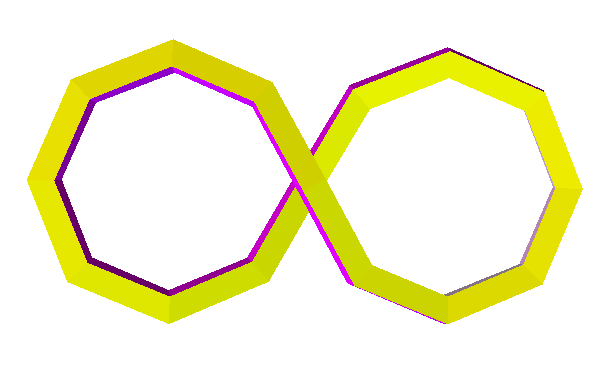
\includegraphics[width=2in]{figure-8-no-twist} & 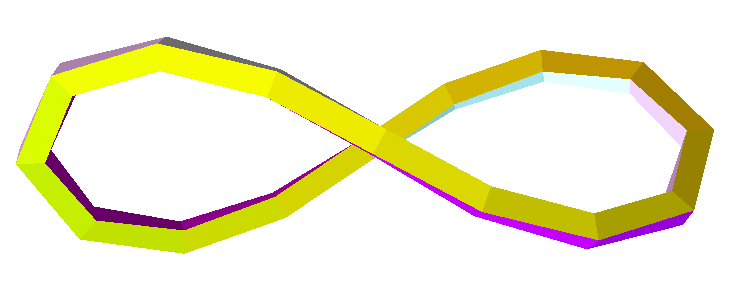
\includegraphics[width=2in]{unfolding-figure-8-1}\tabularnewline
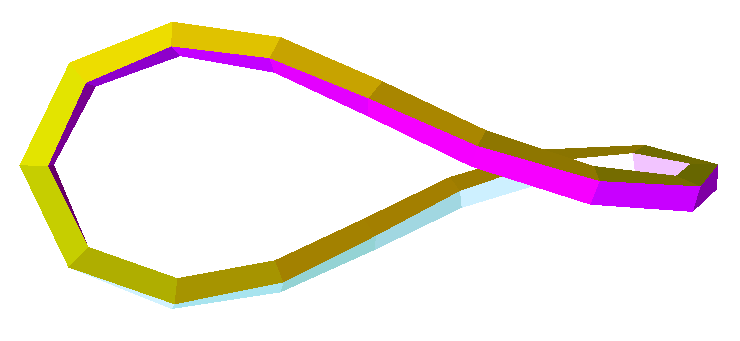
\includegraphics[width=2in]{unfolding-figure-8-2} & 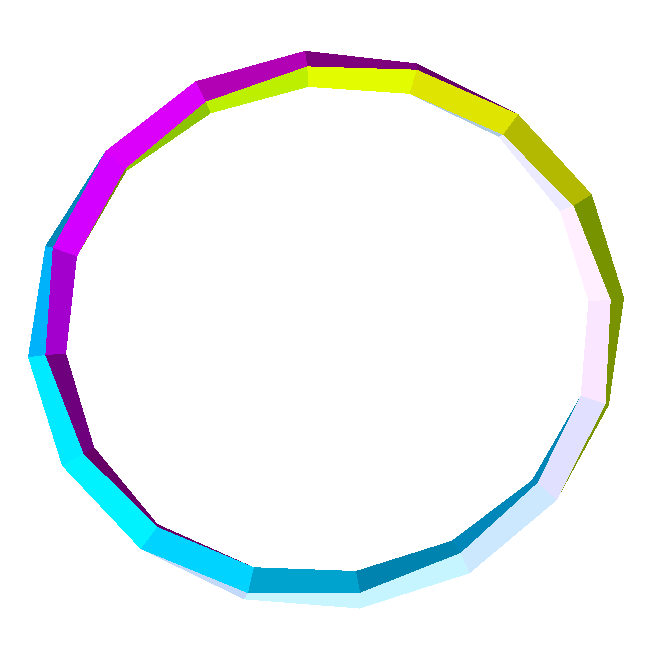
\includegraphics[width=2in]{twisted-circle}\tabularnewline
\end{tabular}\hfill{}

\caption{\label{fig:eight2circle}
Continuous deformation of an untwisted near-planar figure-8 loop into
a twisted planar circle. The shape is rendered so that the individual
control points are easily visible, highlighting the movement of these
points during the transformation.}
\end{figure}



The result of the optimization of this toroid is highly sensitive to
the value of $\alpha$. Empirically, it was determined that for the 16-segment loop 
$\alpha$ values below $0.048324$ resulted in the shape unfolding into
a twisted circle, whereas any value of $\alpha$ larger than this
particular number resulted in very little change from the initial
configuration.

Intermediate configurations between a planar, untwisted figure eight
and a planar, twisted circle were achievable when the input shape contained fewer control points. 
With only 8 control points in the loop and suitable parameter values for $\alpha$, 
the toroid shape manages to find a balance between bending energy,
which is minimized by a circular configuration, and twisting energy,
which is minimized by the figure-8 loop. 
The results correspond to different intermediate states of unfolding of the figure-8 loop (see Figure 6).

\begin{figure}
\hfill{}

\begin{tabular}{cc}
\subfloat[Initial shape: a warped figure-8 loop. Note the low number of control points]{
\includegraphics[width=2in]{alpha-balance-1}

} & \subfloat[$\alpha=0.1$, enough to cause the figure to unfold completely]{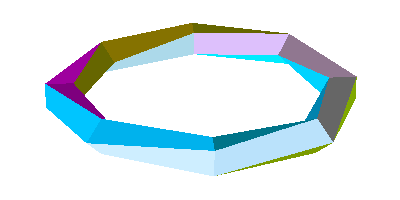
\includegraphics[width=2in]{alpha-balance-2}

}\tabularnewline
\subfloat[$\alpha=0.15$, resulting in an intermediate state]{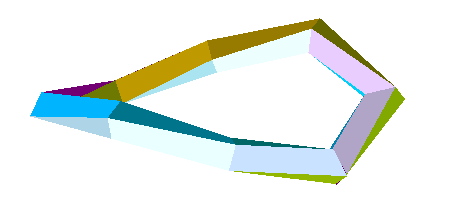
\includegraphics[width=2in]{alpha-balance-3}} & \subfloat[$\alpha=0.2$, enough to prevent any unfolding]{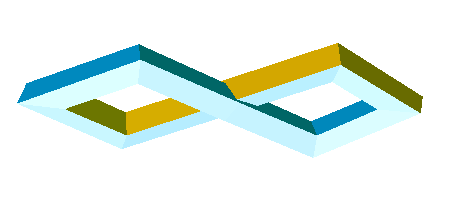
\includegraphics[width=2in]{alpha-balance-4}}\tabularnewline
\end{tabular}\hfill{}

\caption{\label{fig:intermediate_states}
Intermediate states of unfolding in order to balance bending and twisting
energy for different vaues of $\alpha$.}
\end{figure}


Figure 7 demonstrates the inverse of this optimization process.
We start with a nearly circular loop with a user-added twist of $360^{\circ}$.
We also add some perturbation on one side of the circle to break the symmetry of this configuration
and to give the optimization a clear direction in which to start warping the circle
so that it eventually ends up in a figure-8 configuration with no twist at all.

%While a planar circle with a twist of $360^{\circ}$ demonstrated
the limitations of our system, the same shape with a slight perturbation
of one of the control points off the plane in which the other points
lie is indeed correctly optimized, albeit in an undesirable manner.
The perturbation effectively signals to the optimization that some
form of folding out of the plane should occur, but the optimization
proceeds locally before producing the desired planar, untwisted figure
eight. This result is summarized in Figure 7.

\begin{figure}

\hfill{}%
\begin{tabular}{cc}
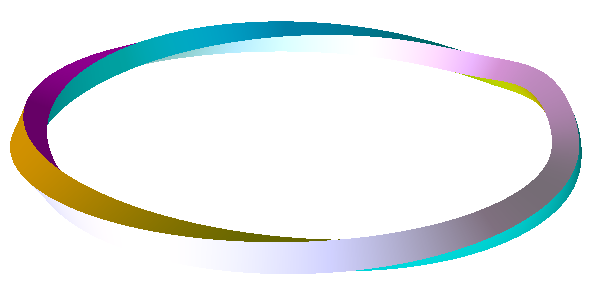
\includegraphics[width=2in]{perturbed-1} & 
\includegraphics[width=2in]{perturbed-2}\tabularnewline
\noalign{\vskip{0.5cm}}
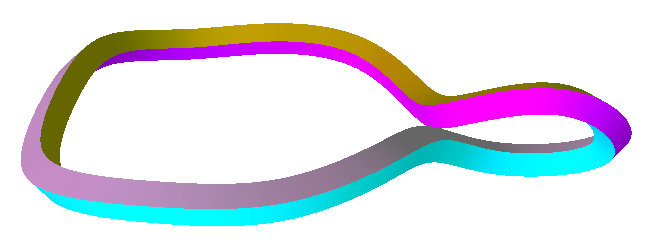
\includegraphics[width=2in]{perturbed-3} & 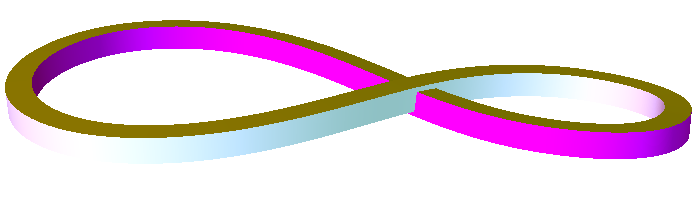
\includegraphics[width=2in]{perturbed-4}\tabularnewline[0.5cm]
\noalign{\vskip\doublerulesep}
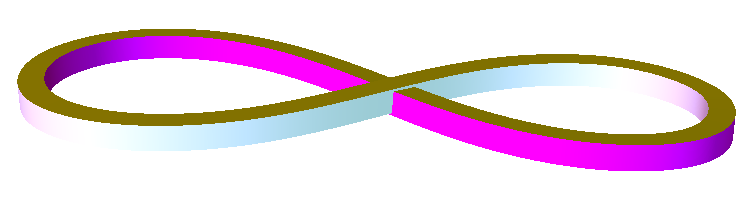
\includegraphics[width=2in]{perturbed-5} & \tabularnewline
\end{tabular}\hfill{}

\caption{\label{fig:circle2eight}
A nearly-planar circle with a twist of $360^{\circ}$ folds itself
into a figure eight. This optimization was performed with $\alpha=0.5$.}

\end{figure}


Next we demonstrate the unfolding of a doubly-looped circle, both with and without an initial twist.
In Figure 8 the double loop has an initial twist of $360^{\circ}$.
Even though it goes through a relatively contorted shape with some pretty sharp bends,
it successfully unfolds itself into a planar, untwisted, single-looped circle when optimized with $\alpha=0.5$.

In Figure 9 the double loop has no twist, but some perturbation to brake the planarity of this configuration.
When optimized under pure bending energy with $\alpha=0$,
it gracefully unfolds into an almost planar figure-8 loop,
and from there into a planar single-looped circle with a twist of $360^{\circ}$,
following the sequence shown in Figure 3.

\begin{figure}
\hfill{}%
\begin{tabular}{cc}
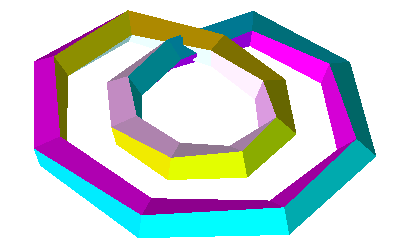
\includegraphics[width=2in]{double-circle-1} & 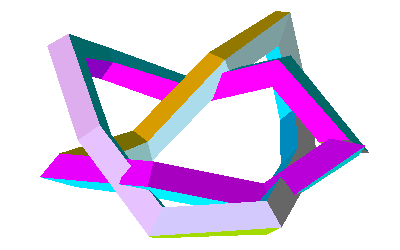
\includegraphics[width=2in]{double-circle-2}\tabularnewline
\noalign{\vskip0.5cm}
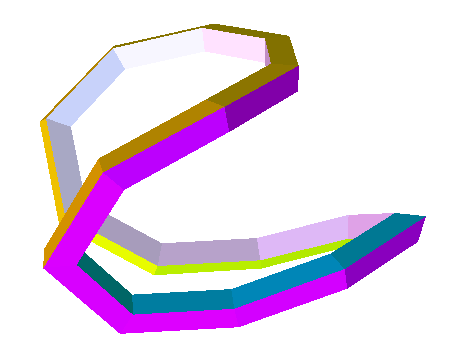
\includegraphics[width=2in]{double-circle-3} & 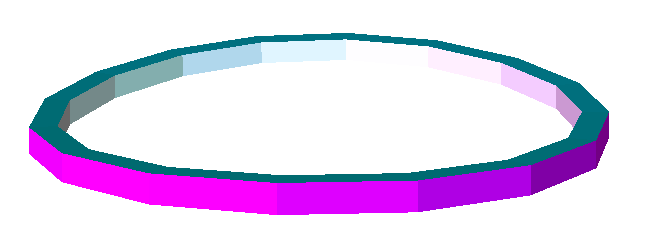
\includegraphics[width=2in]{double-circle-4}\tabularnewline[0.5cm]
\end{tabular}\hfill{}

\caption{A double-looped circle with an initial twist of $360^{\circ}$ unfolds
into a planar, untwisted circle, with $\alpha=0.5$. The camera orientation
differs in each capture to highlight the prominent features in the
intermediate configurations.}
\end{figure}


\begin{figure}
\hfill{}%
\begin{tabular}{cc}
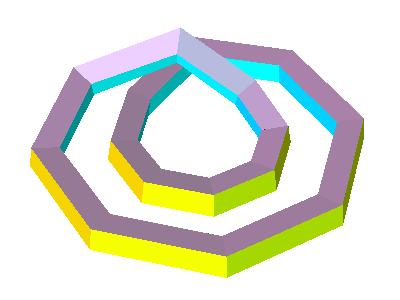
\includegraphics[width=2in]{double-circle-5} & 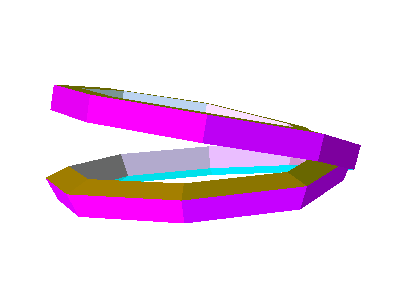
\includegraphics[width=2in]{double-circle-6}\tabularnewline
\noalign{\vskip0.5cm}
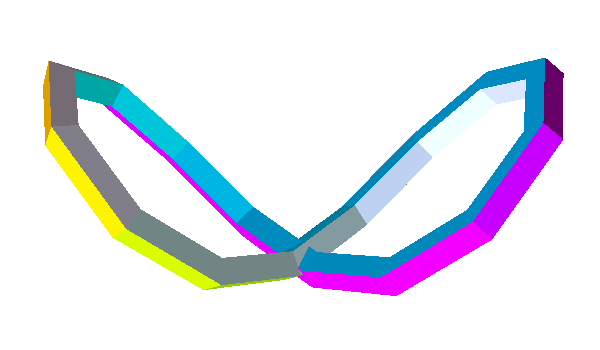
\includegraphics[width=2in]{double-circle-7} & 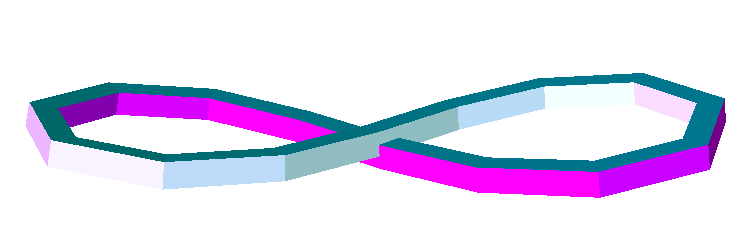
\includegraphics[width=2in]{double-circle-8}\tabularnewline[0.5cm]
\end{tabular}\hfill{}

\caption{A double-looped circle with no initial twist unfolds into a planar,
twisted circle, with $\alpha=0$. The camera orientation differs in
each capture to highlight the prominent features in the intermediate
configurations. The second half of the optimization is omitted, as
it does not differ from Figure 3.}
\end{figure}


\subsection{More Complex Examples}
 
[[ Add a couple of more complex pictures:  e.g. the unwinding of the heavily twisted circle,

and of a 3,4 torus knot with moderate twist - ending up in a circle with 360 deg twist.
-- I will provide a starting path ... ]]



\subsection{Unexpected, Undesirable Behavior}

There were some optimization sequences that surprised us,
and where we first thought that there was something wrong with our torus representation
or with our gradient-descent process.
One such problem sequence is shown in \ref{fig:wiggles}.
We start with a perfectly symmetrical circular loop with 16?? segments and with a twist of $360^{\circ}$.
But his toroid, rather than unfolding into a planar figure-8 loop as in \ref{fig:circle2eight},
ends up in a 4-fold symmetrical hoop with four wavy "sides".
When we monitor the behavior of the various energy components ( \ref{fig:energycurves} ),
we see that the twist energy is reduced dramatically, by a factor of 36,
while there is only a modest increase in bending energy of about a factor of 5.
So what is going on here?

Actually, we could synthesize a perfect, twist-free solution 
with a rectilinear cubist control polygon that produces four planar, S-shaped curve that join together
with four vertical junctions where the Frenet frame makes an instant $90^{\circ}$ turn.
This accommodates an overall twist of $360^{\circ}$ with no twist penalty, 
since all four junctions allow an RMF frame to pass through completely undisturbed.

[[Here are the coordinates for such a control polygon:
(1 1 -1) (1 1 1) (0 1 1) (0 1 -1) (-1 1 -1) (-1 1 1) (-1 0 1) (-1 0 -1) (-1 -1 -1) (-1 -1 1) (0 -1 1) (0 -1 -1) (1 -1 -1) (1 -1 1) (1 0 1) (1 0 -1)
Render a piece-wise linear and/or quadratic B-spline of this loop and insert into \ref{fig:wiggles}. ]]


\begin{figure}
\hfill{}%
\begin{tabular}{ccc}

\includegraphics[width=1.5in]{lim-twisted-circle-1} & 
\includegraphics[width=1.5in]{lim-twisted-circle-2} & 
\includegraphics[width=1.5in]{lim-twisted-circle-3}\tabularnewline
\multicolumn{3}{c}{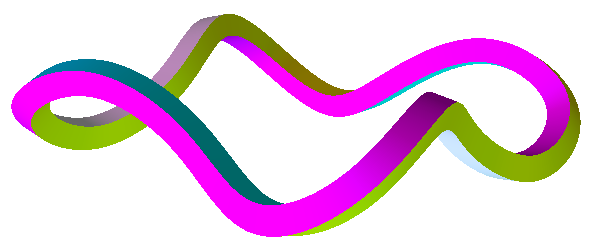
\includegraphics[width=2in]{lim-twisted-circle-4}}\tabularnewline
\end{tabular}\hfill{}

\caption{\ref{fig:wiggles} 
A planar circle with an initial twist of $360^{\circ}$ bends inwards
to minimize its twist. Optimization performed using $\alpha=0.5$.}
\end{figure}


\begin{figure}
\begin{centering}
% GNUPLOT: LaTeX picture with Postscript
\begingroup
  \makeatletter
  \providecommand\color[2][]{%
    \GenericError{(gnuplot) \space\space\space\@spaces}{%
      Package color not loaded in conjunction with
      terminal option `colourtext'%
    }{See the gnuplot documentation for explanation.%
    }{Either use 'blacktext' in gnuplot or load the package
      color.sty in LaTeX.}%
    \renewcommand\color[2][]{}%
  }%
  \providecommand\includegraphics[2][]{%
    \GenericError{(gnuplot) \space\space\space\@spaces}{%
      Package graphicx or graphics not loaded%
    }{See the gnuplot documentation for explanation.%
    }{The gnuplot epslatex terminal needs graphicx.sty or graphics.sty.}%
    \renewcommand\includegraphics[2][]{}%
  }%
  \providecommand\rotatebox[2]{#2}%
  \@ifundefined{ifGPcolor}{%
    \newif\ifGPcolor
    \GPcolortrue
  }{}%
  \@ifundefined{ifGPblacktext}{%
    \newif\ifGPblacktext
    \GPblacktexttrue
  }{}%
  % define a \g@addto@macro without @ in the name:
  \let\gplgaddtomacro\g@addto@macro
  % define empty templates for all commands taking text:
  \gdef\gplbacktext{}%
  \gdef\gplfronttext{}%
  \makeatother
  \ifGPblacktext
    % no textcolor at all
    \def\colorrgb#1{}%
    \def\colorgray#1{}%
  \else
    % gray or color?
    \ifGPcolor
      \def\colorrgb#1{\color[rgb]{#1}}%
      \def\colorgray#1{\color[gray]{#1}}%
      \expandafter\def\csname LTw\endcsname{\color{white}}%
      \expandafter\def\csname LTb\endcsname{\color{black}}%
      \expandafter\def\csname LTa\endcsname{\color{black}}%
      \expandafter\def\csname LT0\endcsname{\color[rgb]{1,0,0}}%
      \expandafter\def\csname LT1\endcsname{\color[rgb]{0,1,0}}%
      \expandafter\def\csname LT2\endcsname{\color[rgb]{0,0,1}}%
      \expandafter\def\csname LT3\endcsname{\color[rgb]{1,0,1}}%
      \expandafter\def\csname LT4\endcsname{\color[rgb]{0,1,1}}%
      \expandafter\def\csname LT5\endcsname{\color[rgb]{1,1,0}}%
      \expandafter\def\csname LT6\endcsname{\color[rgb]{0,0,0}}%
      \expandafter\def\csname LT7\endcsname{\color[rgb]{1,0.3,0}}%
      \expandafter\def\csname LT8\endcsname{\color[rgb]{0.5,0.5,0.5}}%
    \else
      % gray
      \def\colorrgb#1{\color{black}}%
      \def\colorgray#1{\color[gray]{#1}}%
      \expandafter\def\csname LTw\endcsname{\color{white}}%
      \expandafter\def\csname LTb\endcsname{\color{black}}%
      \expandafter\def\csname LTa\endcsname{\color{black}}%
      \expandafter\def\csname LT0\endcsname{\color{black}}%
      \expandafter\def\csname LT1\endcsname{\color{black}}%
      \expandafter\def\csname LT2\endcsname{\color{black}}%
      \expandafter\def\csname LT3\endcsname{\color{black}}%
      \expandafter\def\csname LT4\endcsname{\color{black}}%
      \expandafter\def\csname LT5\endcsname{\color{black}}%
      \expandafter\def\csname LT6\endcsname{\color{black}}%
      \expandafter\def\csname LT7\endcsname{\color{black}}%
      \expandafter\def\csname LT8\endcsname{\color{black}}%
    \fi
  \fi
  \setlength{\unitlength}{0.0500bp}%
  \begin{picture}(5400.00,3780.00)%
    \gplgaddtomacro\gplbacktext{%
      \csname LTb\endcsname%
      \put(1078,704){\makebox(0,0)[r]{\strut{} 0}}%
      \put(1078,985){\makebox(0,0)[r]{\strut{} 2}}%
      \put(1078,1266){\makebox(0,0)[r]{\strut{} 4}}%
      \put(1078,1548){\makebox(0,0)[r]{\strut{} 6}}%
      \put(1078,1829){\makebox(0,0)[r]{\strut{} 8}}%
      \put(1078,2110){\makebox(0,0)[r]{\strut{} 10}}%
      \put(1078,2391){\makebox(0,0)[r]{\strut{} 12}}%
      \put(1078,2672){\makebox(0,0)[r]{\strut{} 14}}%
      \put(1078,2954){\makebox(0,0)[r]{\strut{} 16}}%
      \put(1078,3235){\makebox(0,0)[r]{\strut{} 18}}%
      \put(1078,3516){\makebox(0,0)[r]{\strut{} 20}}%
      \put(1210,484){\makebox(0,0){\strut{} 0}}%
      \put(2156,484){\makebox(0,0){\strut{} 50}}%
      \put(3102,484){\makebox(0,0){\strut{} 100}}%
      \put(4048,484){\makebox(0,0){\strut{} 150}}%
      \put(4994,484){\makebox(0,0){\strut{} 200}}%
      \put(440,2110){\rotatebox{90}{\makebox(0,0){\strut{}Energy}}}%
      \put(3140,154){\makebox(0,0){\strut{}Iteration}}%
    }%
    \gplgaddtomacro\gplfronttext{%
      \csname LTb\endcsname%
      \put(4083,3343){\makebox(0,0)[r]{\strut{}Bending Energy}}%
      \csname LTb\endcsname%
      \put(4083,3123){\makebox(0,0)[r]{\strut{}Twist Energy}}%
      \csname LTb\endcsname%
      \put(4083,2903){\makebox(0,0)[r]{\strut{}Spring Energy}}%
    }%
    \gplbacktext
    \put(0,0){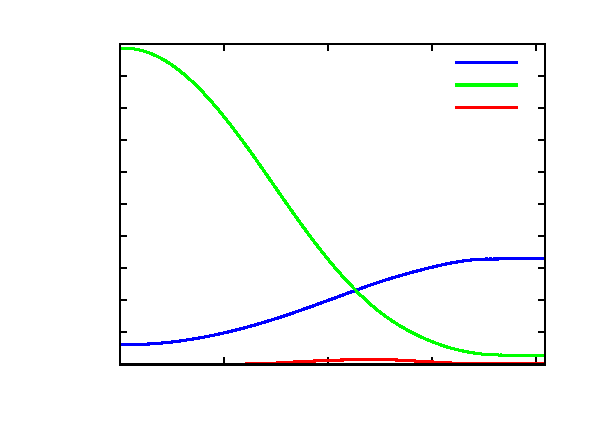
\includegraphics{lim-twisted-circle}}%
    \gplfronttext
  \end{picture}%
\endgroup

\par\end{centering}

\caption{\label{fig:energycurves}
Energy Components for Figure 4 by Iteration}
\end{figure}


This example demonstrates that the use of the overall twist is not sufficient to prevent local twistiness
that may cancel out in the calculation of the overall twist.
Thus we need a more refined measure that captures the twist more locally
and sumes it up in a sign-independent, squared manner.

The problem is, how do we measure such a local twist? 
A natural way would be to determine how much the Frenet frame rotates from one joint to the next;
but this may cause problems for a sequence of nearly collinear line segments,
where a small change in the coordinates of one control point may lead to generation or cancellation of inflection points
Thus the bending angles at the two joints should also be taken into consideration.
This leads to the proposed "non-coplanarity measure" discussed in Section  2.4?? .

Here is a test case that should allow us to analyze how well this new measure resolves this issue of concern:
Connect two multi-looped circles (really helices) and see whether the optimization will unravel this into a simple circle of figure-8 loop.

[[ Control point of "anti-helices":
(2 -1 0.0) (3 0 0.1) (2 1 0.2) (1 0 0.3)  (2 -1 0.4) (3 0 0.5) (2 1 0.6) (1 0 0.7)  (2 -1 0.8) (3 0 0.9) (2 1 1.0) 
(-2 1 1.0) (-3 0 0.9) (-2 -1 0.8) (-1 0 0.7)  (-2 1 0.6) (-3 0 0.5) (-2 -1 0.4) (-1 0 0.3)  (-2 1 0.2) (-3 0 0.1) (-2 -1 0.0) 
--- I am eager to see what happens to this one with old and new functionals !  ]]



\section{Conclusions}

[[some concluding remarks ...]]
With these experiments we have demonstrated that simple CAD models can be constructed 
with suitable cost functions that will evolve toroidal structures to their simplest representative
within the appropriate regular homotopy class.




\section{Acknowledgements}

We would like to thank Satish Rao and Umesh Vazirani for providing
valuable insight regarding gradient descent, and Carlo S�quin, without
whose advice and guidance, this project would not have been possible.



\section{More References}

% TODO
%line search algorithm \cite{??}, 

\bibliographystyle{plain}
\bibliography{references}

\end{document}
